\documentclass[tikz,border=3mm]{standalone}
\usepackage{pgfplots}
\pgfplotsset{compat=1.17}
\usepgfplotslibrary{groupplots}
\usetikzlibrary{arrows.meta,positioning,fit,shapes.geometric,calc,backgrounds}
\begin{document}

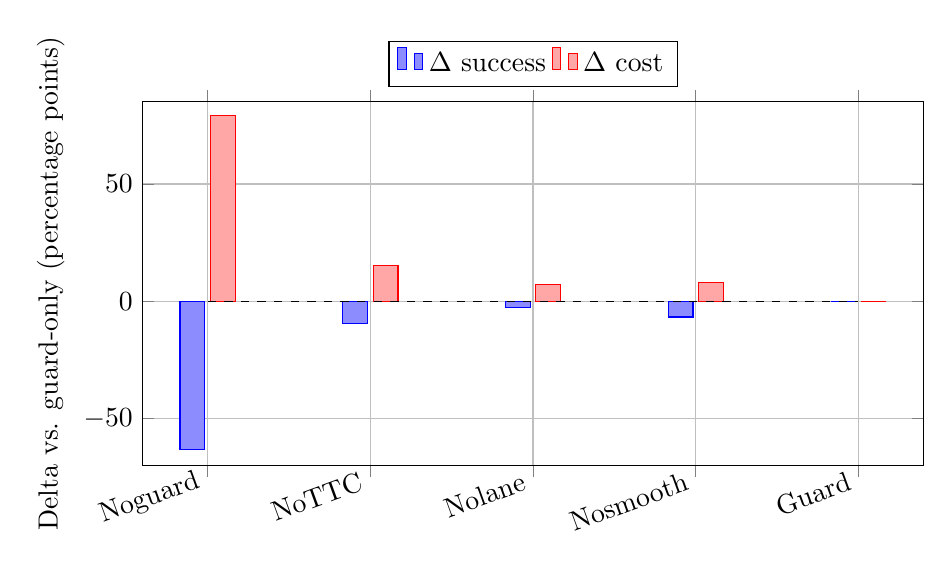
\begin{tikzpicture}
\begin{axis}[width=11.5cm,height=6.2cm,ybar,bar width=9pt, symbolic x coords={Noguard,NoTTC,Nolane,Nosmooth,Guard}, xtick=data, x tick label style={rotate=20,anchor=east}, ylabel={Delta vs. guard-only (percentage points)}, ymin=-70, ymax=85, grid=major, legend style={at={(0.5,1.04)},anchor=south,legend columns=2}]
\addplot+[fill=blue!45] coordinates {(Noguard,-63.3) (NoTTC,-9.3) (Nolane,-2.7) (Nosmooth,-6.7) (Guard,0.0)}; \addlegendentry{$\Delta$ success}
\addplot+[fill=red!35] coordinates {(Noguard,79.3) (NoTTC,15.3) (Nolane,7.3) (Nosmooth,8.0) (Guard,0.0)}; \addlegendentry{$\Delta$ cost}
\draw[dashed] (axis cs:Noguard,0)--(axis cs:Guard,0);
\end{axis}
\end{tikzpicture}

\end{document}
